\chapter{Grundlagen} % (fold)
\label{sec:grundlagen}
Die folgenden Abschnitte sollen die theoretischen Grundlagen vermitteln, die notwendig sind, um das Thema dieser Thesis zu betrachten. Die Konzepte, die hier beschrieben werden sind API-Grundlagen, REST und GraphQL.
\section{API Grundlagen} % (fold)
\label{sec:apigrundlagen}
Nachfolgend werden die Grundlagen von APIs thematisiert. Hierbei werden die grundlegenden Definitionen im Zusammenhang mit APIs und die verschiedenen Typen vorgestellt.
\subsection{Grundlegende Definition von API} % (fold)
\label{sec:grundlegendedefinitionvonapi}
Der Begriff \glqq API\grqq{}  steht für \glqq Application Programming InterfaceI\grqq{}. Eine API bezeichnet eine Schnittstelle, welche Entwicklern den Zugriff auf Daten und Informationen ermöglicht. Bekannte Beispiele für häufig genutzte APIs sind die Twitter- und Facebook-APIs. Diese sind für Entwickler zugänglich und ermöglichen die Interaktion mit der Software von Twitter und Facebook. Zudem ermöglichen APIs die Kommunikation zwischen Anwendungen. Sie bieten den Anwendungen einen Weg, miteinander über das Netzwerk, überwiegend das Internet, in einer gemeinsamen Sprache zu kommunizieren. \citep{apistrategyguide}
\newpage
%subsection grundlegendedefinitionvonapi (end)
\subsection{API Typen} % (fold)
\label{sec:apitypen}
APIs können anhand von Verfügbarkeit, Anwendungszweck oder der Spezifikation in verschiedene Typen eingeteilt werden.

\subsubsection{API Typen nach Verfügbarkeit} % (fold)
\label{sec:apitypenverfuegbarkeit}
Im Bezug auf Verfügbarkeit können APIs public (öffentlich), privat oder für Partner bereitgestellt werden. 
\citep{apimindset}
\begin{figure}[h!]
	\centering
	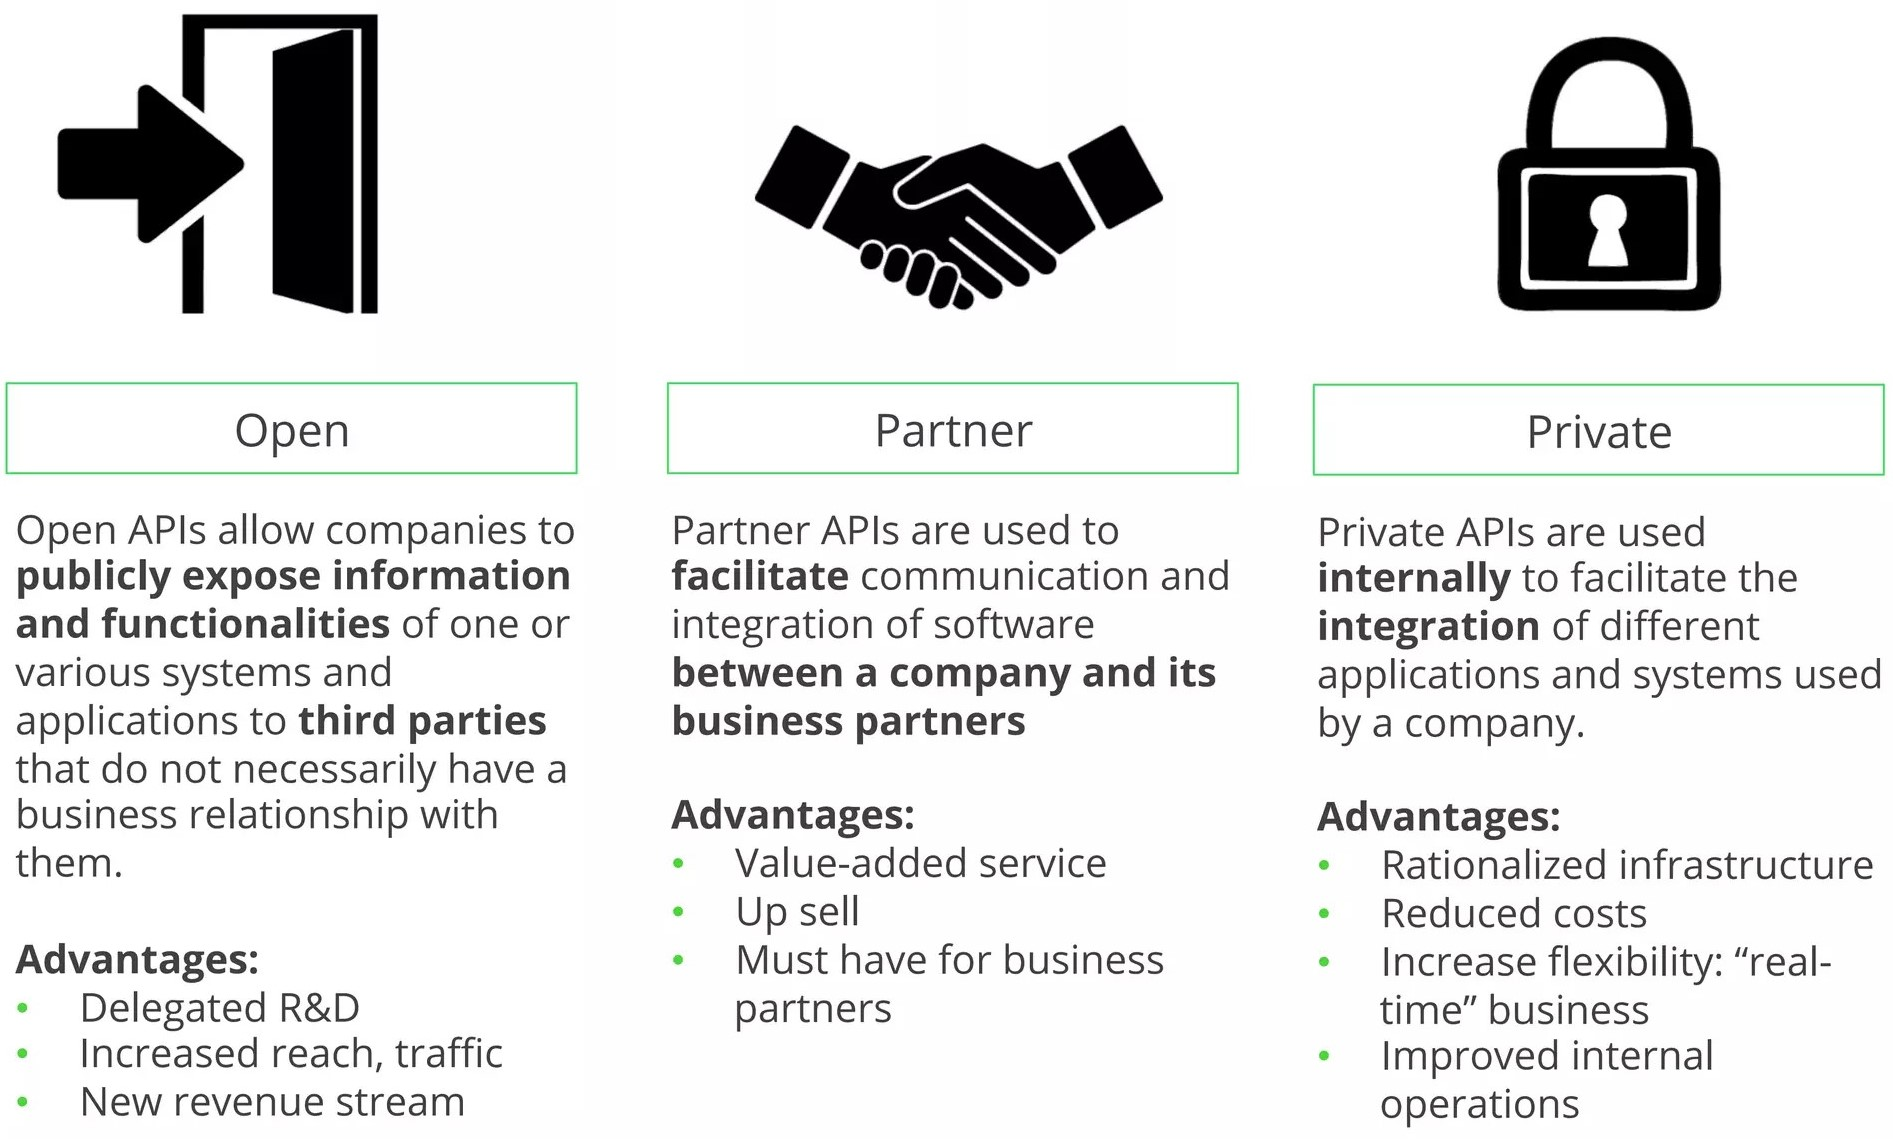
\includegraphics[scale=0.225]{Illustrations/apitypes.jpg}
	\caption{API Typen nach Verfügbarkeit \citep{graficapitypes}}
\end{figure}

\begin{itemize}
	\item \textbf{Public APIs:} Öffentliche APIs sind für jeden Entwickler bzw. jegliche Dritte verfügbar. Eine Public API erhöht die Markenbekanntheit und kann bei Monetarisierung zusätzliche Einkommensmöglichkeiten bieten. \citep{apimindset}
	\item \textbf{Privat APIs:} Dieser Typ ermöglicht firmeninternen Entwicklern die Nutzung der API zu Integration interner Produkte, Systemen oder Apps. Zudem können bei der Entwicklung von neuen Systemen bestehende Ressourcen genutzt werden. Hierbei entsteht eine erhebliche Kostenersparnis und es besteht eine größere Flexibilität. \citep{apimindset}
	\item \textbf{Partner APIs:} Partner APIs bilden den Schnitt aus privaten und öffentlichen APIs. Sie sind dazu bestimmt die Entwicklung von Anwendungen zwischen Unternehmen zu unterstützen. Die Unternehmen haben dabei eine hohe Nutzerkontrolle.\citep{apimindset}
\end{itemize}
%subsubsection apitypenverfuegbarkeit (end)

\subsubsection{API Typen nach Anwendungszweck} % (fold)
\label{sec:apitypenanwendungszweck}
\begin{itemize}
\item \textbf{Datenbanken APIs} ermöglichen die Kommunikation zwischen einer Datenbank und einer Anwendung die deren Daten benötigt. \citep{TUM}

\item \textbf{Betriebssystem APIs} definieren wie Ressourcen und Services von Betriebssystemen von einer Anwendung benutzt werden, die auf deren Daten zugreift. \citep{TUM}

\item \textbf{Remote APIs} definieren die Regeln, wie Anwendungen auf verschiedenen Host-Maschinen miteinander interagieren. \citep{TUM}

\item \textbf{Web APIs} sind die verbreitetsten APIs. Sie stellen Daten bereit und übermitteln diese zwischen Web-basierenden Systemen über eine Client-Server Verbindung. \citep{TUM}

\end{itemize}
%subsubsection apitypenanwendungszweck (end)

\subsubsection{API Typen nach Spezifikation/Protokoll} % (fold)
\label{sec:apitypenspezifikation}
Das Ziel der Spezifikation von APIs ist die Kommunikation zwischen verschiedenen Services zu standardisieren

\begin{itemize}

	\item \textbf{Remote Procedure Call (RPC)} stellt eine einfache und zugleich die älteste Form von Application Programming Interfaces dar. Ihr Zweck besteht in der Initiierung von Prozeduren auf anderen Systemen. Zu diesem Zweck übermittelt eine Anwendung eine oder mehrere Nachrichten an eine andere Anwendung, um eine Prozedur zu starten. Im Anschluss daran sendet die empfangende Anwendung dem Sender eine oder mehrere Nachrichten zurück, sobald die Prozedur abgeschlossen ist. 
	\citep{TUM}

	\item \textbf{Simple Object Access Protocol (SOAP)} wurde von Microsoft entwickelt und stellt ein leichtgewichtiges Protokoll für den Austausch von Informationen in einer dezentralen, verteilten Umgebung dar. SOAP basiert auf XML und besteht aus einem Umschlag, der den Rahmen für die Beschreibung des Inhalts einer Nachricht und ihrer Verarbeitung definiert, einer Reihe von Kodierungsregeln zur Darstellung von anwendungsdefinierten Datentypen sowie einer Konvention zur Darstellung von Remote-Prozeduraufrufen und Antworten. SOAP wird in erster Linie eingesetzt, um eine sichere Übertragung von Daten zu gewährleisten, und findet insbesondere bei Unternehmen, die Zahlungsgateways, Identitätsmanagementlösungen und Finanzdienstleistungen anbieten, Verwendung.
	\citep{TUM}
\newpage
	\item \textbf{Representational State Transfer (REST)} wurde erstmals im Jahr 2000 in einer Dissertation von Roy Fielding beschrieben. Hierbei handelt es sich um einen Software-Architekturstil für APIs. REST basiert auf einer Ressourcenorientierung, bei der jede Entität als Ressource betrachtet und durch eine eindeutige Uniform Resource Locator (URL) identifiziert wird. Die Architektur basiert auf sechs grundlegenden Beschränkungen, darunter die Client-Server-Architektur, bei der Client und Server unabhängig voneinander agieren. Ein wesentliches Charakteristikum von REST ist die Zustandslosigkeit, d. h. jede Anfrage beinhaltet sämtliche für die Verarbeitung erforderlichen Informationen, wodurch die Interaktion zwischen Client und Server vereinfacht wird. Die Umsetzung der CRUD-Operationen (Create, Read, Update, Delete) erfolgt durch die HTTP-Methoden (POST, GET, PUT, DELETE). REST nutzt das in HTTP integrierte Caching, um die Antwortzeiten und die Leistung zu optimieren. Dabei besteht die Möglichkeit, Serverantworten als cachefähig oder nicht cachefähig zu kennzeichnen. Des Weiteren ist eine einheitliche Schnittstelle zu nennen, welche die Interaktionen zwischen unterschiedlichen Geräten und Anwendungen erleichtert und sichtbar macht. Darüber hinaus erfordert REST ein mehrschichtiges System, bei dem jede Komponente lediglich mit der unmittelbar vorgelagerten Schicht interagiert. Die Bereitstellung von ausführbarem Code durch den Server ist optional. RESTful APIs, die diesen Prinzipien folgen, nutzen HTTP-Anfragen, um Ressourcen effizient zu bearbeiten. \citep{Fielding2000}  \citep{graphqlreplacerest}

	\item \textbf{GraphQL} wurde 2012 von Facebook für den internen Gebrauch entwickelt. Im Jahr 2015 erfolgte die Veröffentlichung als Open-Source-Projekt für die Allgemeinheit. Das Kernkonzept von GraphQL basiert auf client-getriebenen Abfragen, bei denen der Client die Struktur der Daten präzise definiert und nur die erforderlichen Daten erhält. Dies resultiert in einer Reduktion von Datenübertragungen und ermöglicht effizientere Netzwerkaufrufe. Die hierarchische Struktur der Abfragen, welche die Graph-Struktur widerspiegelt, erlaubt eine intuitive Datenmodellierung. Die starke Typisierung in GraphQL wird durch ein Schema definiert, welches die Typen der Daten spezifiziert. Dadurch wird eine bessere Validierung und Dokumentation ermöglicht. Im Gegensatz zu REST, bei dem für verschiedene Operationen mehrere Endpunkte erforderlich sind, verwendet GraphQL lediglich einen einzigen Endpunkt für alle API-Abfragen.  \citep{graphqlreplacerest}

\end{itemize}
%subsubsection apitypenspezifikation (end)
%subsection apitypen (end)

% section apigrundlagen (end)

\newpage
\section{Datenbank Grundlagen} % (fold)
\label{sec:datenbankGrundlagen}
Im Folgenden werden die Grundlagen von Datenbanken behandelt. Es werden grundlegende Definitionen im Zusammenhang mit Datenbanken und die verschiedenen Arten von Datenbanken vorgestellt.
\subsection{Definition Datenbank} % (fold)
\label{sec:definitiondatenbank}
%subsubsection definitiondatenbank (end)

\subsection{Datenbanktypen} % (fold)
\label{sec:datenbanktypen}
%subsubsection datenbanktypen (end)


% section datenbankGrundlagen (end)

% chapter grundlagen (end)